\chapter{研究发现}

在对找到的能实现路况图像风格变换的各个模型进行实验,并得到各个模型的合成图数据后,我们展开了对最后的8个模型实验数据的分析和总结工作。希望最终对数据的观察和分析得出的结论能帮助从事自动驾驶系统测试的技术人员回答以下问题:适合自动驾驶系统测试用例生成的对抗生成网络和神经风格迁移技术的路况图像实际合成效果如何?各个模型的实际训练效率如何?哪个或哪几个深度学习模型总体是最适合自动驾驶系统测试用例的自动生成?

\section{评价指标}

为了对最终的实验数据作更好的总结,我们希望对每个模型从合成图质量、模型训练时间成本以及每个模型对自动驾驶系统的干扰程度分别作出评估,基于以上考虑,我们找到了以下3个评价指标。

\subsection{Fr\'{e}chet Inception Distance(FID)}

对于图像驾驶场景合成图的质量好坏,最直观也是最直接的方式就是比较合成图的视觉效果,但这种人为的评判是主观且十分容易误判的。为了能够客观、量化的比较各个DNN框架合成的驾驶场景图的好坏,学术界提出了两个指标:\textit{Inception Score(IS)}\cite{IS}和\textit{Fre ́chet Inception Distance(FID)}\cite{FID}。

\textbf{Inception Score(IS).\cite{IS}}\quad Inception Score是Goodfellow等人第一次提出能够比较两组图片相似度的一个量化指标。它主要针对对抗生成网络和原数据和其合成数据之间的差异度测量。IS评价合成图片质量是基于以下两点:(i) 包含有意义的物体图像的条件标记分布应该具有较低的熵(entropy)和(ii) 图像的多样性应该较高,进而边缘分布$\int_z p(y|x=G(z))dz$应该有较高的熵。
将以上两点汇总成一个评分,
\begin{gather}
    IS(G)=\exp{(E_{x\sim G}[d_{KL}(p(y|x), p(y)])}
\end{gather}
IS的作者用ImageNet\cite{ImageNet}的数据训练了一个分类器,最终实验结果反映IS的分数与人工标注评价正相关。

\textbf{Fr\'{e}chet Inception Distance(FID).\cite{FID}}\quad FID通过比较真实样本与合成样本的统计数据来改进IS。它提出了另一个评价方法,它首先将所有的合成图片放入一个特征空间,然后将该空间视为一个多元高斯分布,分别计算合成图和真实图的均值与方差,将两者高斯分布的Fre ́chet距离来量化真实图与合成图之间的距离,进而作为对合成图的评价:
\begin{gather}
    FID(x,g)=||\mu_x-\mu_g||_2^2+Tr(\sum_x + \sum_g - 2(\sum_x\sum_g)^{\frac{1}{2}})
\end{gather}
这里的$(\mu_x,\sum_x)$和$(\mu_g,\sum_g)$分别是数据分布和模型分布的均值和方差。FID的作者发现FID值与人类对合成图像的判断一直,并且较IS\cite{IS}鲁棒性更强。相对于IS,FID还能检测出不同类之间的区别,即如果每一种类别值产生合成一张图片,则很有可能获得比较高的IS分数,但对应的FID值却很低。此外,计算FID时用到了合成数据与真实数据,比IS更加合理。总体来讲,FID得分越低越好,对应于合成样本与真实样本之间通过FID测量的距离越短。

基于以上几点,我们选用FID值而不选择IS值作为我们后面实验评价合成图片质量的评价指标之一。

\subsection{模型训练时长}

除了直接比较合成图片质量的好坏,在实际的自动驾驶系统测试过程中,我们还必须考虑到模型的训练时长。在选择理想的图片合成框架时,除了最终合成图片质量的好坏,我们还希望模型的训练时间成本尽可能的小,不同的模型根据不同的训练数据集大小,最终的训练时长也相差越大,比如本章后面会提到的UNIT\cite{UNIT}基于Udacity自动驾驶数据集\cite{udacity_dataset}和大约3000张驾驶场景图片,训练50万次时长大约一周左右。而对于一些图像风格转换(Neural Style Transfer)模型来说,训练时长却只要几个小时,虽然最后合成图的质量不如UNIT,但我们希望把这些数据都统计出来,具体的取舍留给实际最终的测试人员自己选择。 

\subsection{方向盘拐角差}

有了合成图质量的量化指标,模型的训练时间成本,最后我们还希望直观地看到合成图相比原始图对于自动驾驶系统行为判断的干扰。方向盘控制信号作为目前学术界研究自动驾系统主要考虑的输出信号,因此我们将自动驾驶系统输出的方向盘拐角值作为自动驾驶系统的主要输出值。另一方面,我们引用了DeepRoad测试框架使用的蜕变测试概念,质量合格的合成图与原图应该存在着蜕变关系,因此我们期待自动驾驶系统对于两者的输出趋于一致,即理想情况下,只变换驾驶场景图片的风格,比如晴天的路况转换为夜晚、雨天或者阴天的路况,自动驾驶系统对于大部分的转换后的图像的行为判断,即输出的方向盘拐角信号,与原始的驾驶路况图片做出的行为判断应该几乎一致,或者差别不大。实验中我们参照DeepRoad测试框架,对两者的信号差别,即拐角差设置了一个阈值$\alpha=5^{\circ}$,统计了拐角差超过阈值的行为数,即DeepRoad里面统计的自动驾驶系统行为不一致数,从模型比较的角度观察,该指标反应了模型合成图对于自动驾驶系统的干扰度。

\section{实验数据统计}

\textbf{训练时长.}\quad 在将我们找到的能够实现驾驶场景图片转换功能的模型基于Udacity自动驾驶数据集\cite{udacity_dataset}和已有的从Youtube上爬取的数据集进行图像转换实验,且得到各个模型的合成图数据后,我们首先统计的指标是各个模型的\textbf{训练时长}。所有模型的训练平台硬件环境都一致,主要配置参数为:Ubuntu 16.04 LTS操作系统,8核GeForce GTX 1080ti GPU,8核Intel(R) Core(TM) i7-6700 CPU。统计训练时长的工具使用的是GNU开源工具\textit{time},各个模型训练耗时数据如下表\ref{table:time}所示:

\begin{table}[h]
    \centering
    \caption{模型训练时间统计表}
    \begin{tabular}{l{3.5cm}rrr}
        \toprule
        \mthead{模型名称} & \mthead{real} & \mthead{user} & \mthead{sys} \\
        \midrule
        MUNIT & 3743m77.651s & 4927m93.474s & 837m.52.196s \\
        % \hline
        CycleGAN & 3154m38.274s & 4081m81.696s & 731m20.894s \\
        % \hline
        EBGAN & 3811m24.172s & 5021m32.721s & 757m19.141s \\ 
        % \hline
        AdaIn Style & 2349m46.212s & 3782m18.764s & 554m26.476s \\ 
        % \hline
        Deep Photo Style Transfer & \multicolumn{3}{c}{\textit{pre-trained}} \\ 
        % \hline
        Fast Photo Style & \multicolumn{3}{c}{\textit{pre-trained}} \\ 
        % \hline
        Fast Neural Transfer & \multicolumn{3}{c}{\textit{pre-trained}} \\ 
        % \hline
        Texture Nets & \multicolumn{3}{c}{\textit{pre-trained}} \\ 
        % \hline
        \bottomrule
    \end{tabular}
    \label{table:time}
\end{table}

\textbf{FID.}\quad 我们参考了文献\cite{FID}提供的FID计算算法,利用Pytorch库对算法进行了实现并最终计算了8个模型合成图的fid值,下表\ref{table:fid}为所有模型的FID值统计数据:

\begin{table}[h] 
    \centering
    \scriptsize
    \caption{FID值统计表}
    \begin{tabular}{l*{4}{p{2.5cm}}}
        \toprule
        模型 & MUNIT & CycleGAN & EBGAN & AdaIN Style & Deep Photo Style & Fast Photo Style & Fast Neural Transfer & Texture Nets \\
        \midrule
        FID值 & 185.18924 & 275.04948 & 217.82906 & 88.39498 & 77.28563 & 139.49777 & 92.61378 & 87.31297  \\
        \bottomrule
    \end{tabular}
    \label{table:fid}
\end{table}

\textbf{方向盘拐角.}\quad 为了测出每个模型最终的合成图对自动驾驶系统的干扰,即合成图的拐角与原图的拐角差,实验中自动驾驶拐角预测模型我们使用了Udacity自动驾驶竞赛中的cg23\cite{cg23}模型。由于模型代码的限制,在输出拐角前还必须对已有的合成图做相应的时间戳标记,这一部分使用了Udacity Driving Reader代码\cite{git:udr}。期间,由于作者提供的最初的实验代码中有大量是基于Udacity自动驾驶竞赛定制的代码,无法很好的移植到我们的实验中,于是在参考了其他代码后我们融合了cg23和该竞赛中其他模型的拐角预测代码,整体模型是基于Tensorflow构造的6层卷积神经网络实现的。得到了所有图片在自动驾驶系统下的方向盘拐角预测值后,为了显示出其与原始图片在自动驾驶系统下的预测拐角值偏差,我们计算了所有单张图与原图拐角差值的平均方差,以此来总体评价合成图对自动驾驶系统的干扰。最终我们使用Python的Matplotlib库将差值数据可视化的绘制在图表上。

图5-1到图5-8是8个实验模型最终的拐角偏差数据,图中红色是原图在自动驾驶中的拐角,蓝色是合成图的拐角差,横轴是原图名称,即Udacity原始数据集单张图像拍摄的时间戳。

\begin{figure}[!h]
    \includegraphics[width=1.5\textwidth, center]{rmse/1} 
    \caption{MUNIT}
\end{figure}
\begin{figure}[!h]
    \includegraphics[width=1.5\textwidth, center]{rmse/2} 
    \caption{CycleGAN}
\end{figure}
\begin{figure}[!h]
    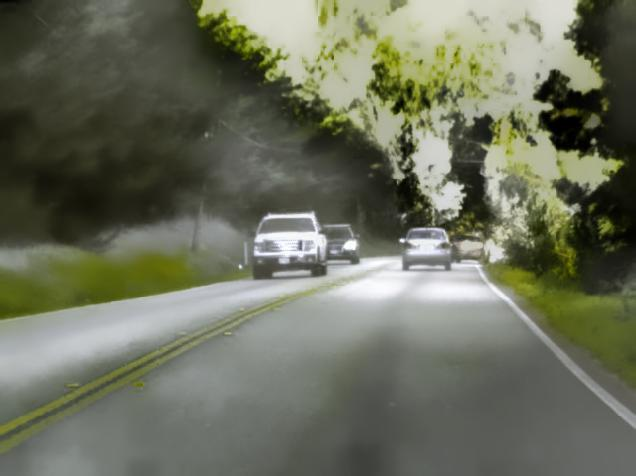
\includegraphics[width=1.5\textwidth, center]{rmse/3} 
    \caption{EBGAN}
\end{figure}
\begin{figure}[!h]
    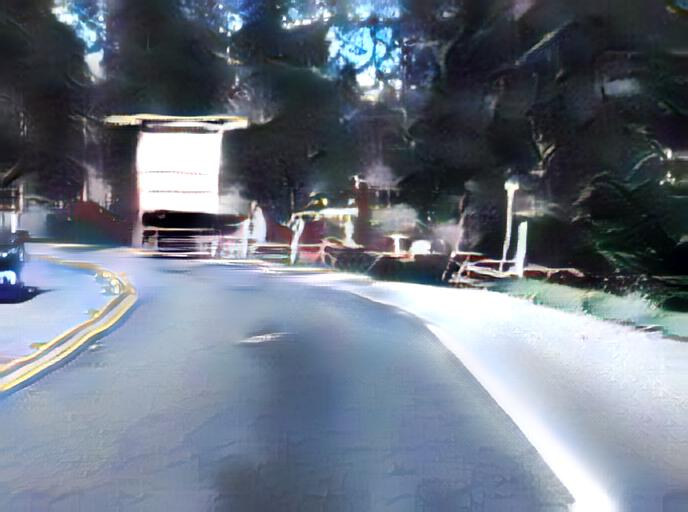
\includegraphics[width=1.5\textwidth, center]{rmse/4} 
    \caption{AdaIN Style}
\end{figure}
\begin{figure}[!h]
    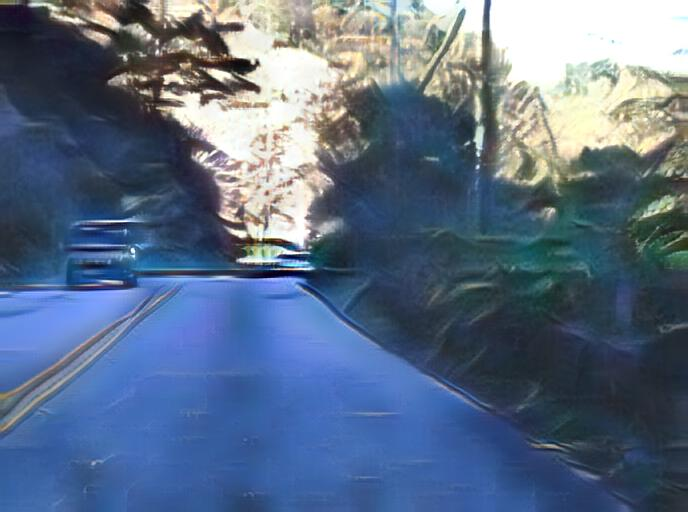
\includegraphics[width=1.5\textwidth, center]{rmse/5} 
    \caption{Deep Photo Style}
\end{figure}
\begin{figure}[!h]
    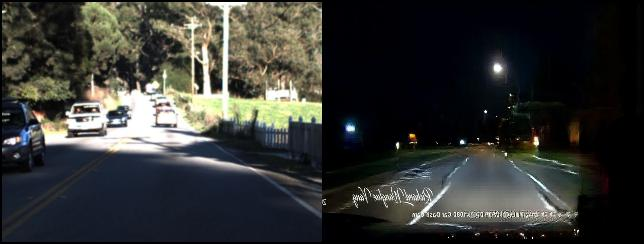
\includegraphics[width=1.5\textwidth, center]{rmse/6} 
    \caption{Fast Photo Style}
\end{figure}
\begin{figure}[!h]
    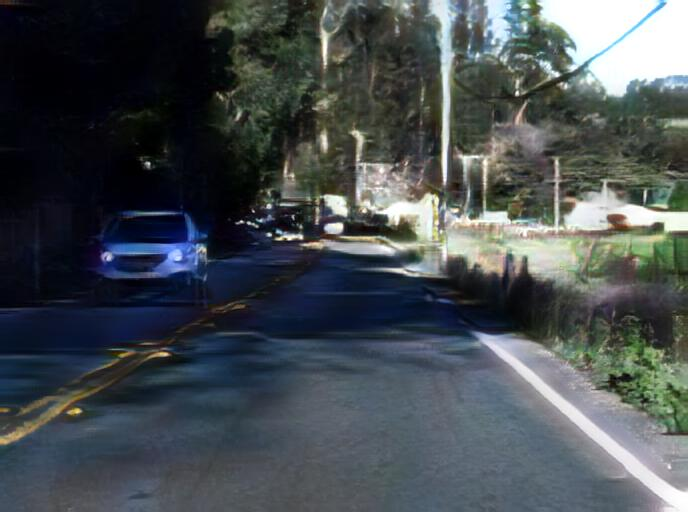
\includegraphics[width=1.5\textwidth, center]{rmse/7} 
    \caption{Fast Neural Transfer}
\end{figure}
\begin{figure}[!h]
    \includegraphics[width=1.5\textwidth, center]{rmse/8} 
    \caption{Texture Nets}
\end{figure}

\section{定量发现分析}

为了对统计的实验数据有更为直观的认识,我们根据表\ref{table:fid}和方向盘拐角差方差值画了柱状图,如图\ref{fig:col}所示,通过对训练时长统计表\ref{table:time}和FID、方向盘拐角差数据的直接观察,我们有以下发现:

\begin{figure}[ht]
    \centering
    \subfigure[FID数据柱状图]{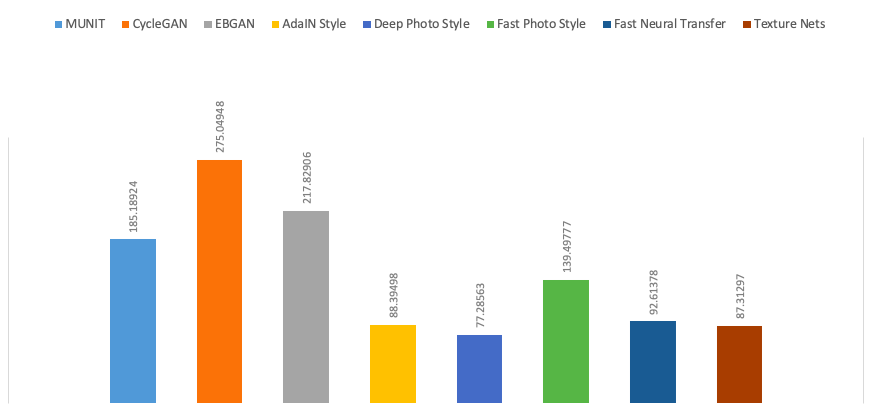
\includegraphics[width=\textwidth]{col_fid}}
    \subfigure[方向盘拐角方差数据柱状图]{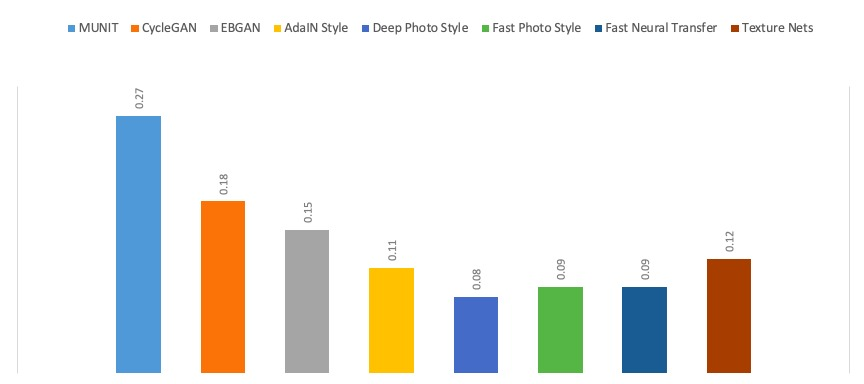
\includegraphics[width=\textwidth]{col_sad}}
    \caption{FID和方向盘拐角方差数据柱状图}
    \label{fig:col}
\end{figure}

% TODO item标号改为 发现1\2\3...
\begin{enumerate}[itemindent=40pt, listparindent = 0.7cm, label={发现\arabic*:}]
    \item \textbf{对抗生成网络技术的模型训练时间成本高于神经风格迁移技术}
    
    主要原因在与大部分的神经风格迁移技术(Adain Style除外),都是将事先基于ImageNet数据集识别任务训练好的VGG-19网络模型直接用于输入图像的特征提取和数据分布学习,图像合成的任务只需在原有的网络模型结构中增加对提取的图像特征进行重构还原的全连接层即可,一般只需添加2层。对于新添加的网络层参数学习时长对比对抗生成网络中的整个模型训练时长可以忽略不计。
    
    具体的,在实验过的模型中,模型训练时间成本最高的是MUNIT,CycleGAN和EBGAN,因此我们建议在时间不充裕的情况下可以优先考虑使用神经风格迁移技术的模型,对于模型风格不同的需求可以通过更换提前训练好的模型网络来实现,而无需想对抗生成网络一样对新数据重新进行一遍整体模型的训练。尽管大部分神经风格迁移技术有无需对整体模型进行训练的便利,但我们在实验中发现神经风格迁移技术对单张图片的转换时间比训练好的对抗生成网络模型耗时要更长,一般训练好的对抗生成网络模型单张图片合成平均耗时约5秒左右,而我们统计的神经风格迁移技术依具体模型不同耗时在1分钟到20分钟。因此如果考虑到实时图形转换,譬如视频实时合成的需求,则对抗生成网络大类的技术是更好的选择。 

    \item \textbf{神经风格迁移技术合成图与原图更接近}
    
    从FID数据柱状图\ref{fig:col}可以明显地看出对抗生成网络类模型的FID得分普遍比神经风格迁移技术的得分要差,由FID值的含义可知,神经风格迁移技术的合成图要比对抗生成网络的合成图更接近与原图。我们试图对这种现象做出解释:神经风格迁移技术的训练网络大多都使用了典型的VGG-19网络,比如文献\cite{nst}中提出的算法使用的网络为基于ImageNet数据集\cite{ImageNet}上训练好的VGG网络,算法使用该网络对图像进行特征提取工作,根据卷积神经网络的特性:卷积层越高,提取的特征也就越抽象,因此神经风格迁移技术将网络中高层的Feature Map信息保存,作为图像的内容特征,以此在图像合成阶段重构图像的内容信息。 

    另一方面,图像的风格特征是通过求各个卷积层卷积核,即过滤器的协方差得到。每层卷积层的卷积核之间的协方差描述了图像的纹理及颜色信息,通过求出每层卷积层卷积核之间的协方差可以构建出图像的特征空间,并通过该空间将图像风格信息进行重建。

    神经风格迁移技术正是通过上述方式将图像的内容信息和风格信息分别提取出来,然后再图像重构阶段对不同的内容空间和风格空间的元素进行重组,从何实现图像的风格变化。而大部分的对抗生成网络技术一般没有对原图像进行风格信息和内容信息的分开提取,图像合成机制主要是靠传统的生成器和判别器协作对抗完成,因此合成图像对于原图像的内容信息保留较神经风格迁移技术而言,要少得多,进而导致合成图与原图的差别要大于神经风格迁移技术的合成图与原图的差别。

    \begin{figure}[h]
        \centering
        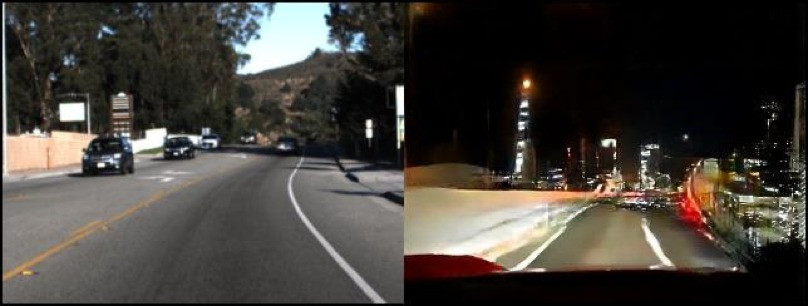
\includegraphics[width=.32\textwidth]{gan_bad}
        \includegraphics[width=.32\textwidth]{models/EBGAN/8}
        \includegraphics[width=.32\textwidth]{models/GAN/1}
        \caption{MUNIT合成图像样本}
        \label{fig:gan}
    \end{figure}
    
    大部分的对抗生成网络技术中,合成数据的质量主要依赖于系统中的生成器对于原始数据分布的学习能力,以图像数据的生成为例,生成器在学习原图像数据分布时并没有对远图像的语义和风格信息作特殊处理,对图像内容的语义信息也没有类似于语义分割的处理,它是将原图像数据当做一个整体进行数据分布的学习,因此往往会导致最后判别器产生的合成图是对原始图的全盘模拟,特别的当输入数据由风格图和内容图两张图组成时,合成图会展现出两者的综合效果,例如图\ref{fig:gan}展示的,可以发现合成图不仅有白天的道路信息,风格图存在而原图中不存在的建筑、路灯信息却大量地出现在了合成图中。
    
    虽然从合成图与原图相似度上看,对抗生成网络技术的性能不如神经风格迁移技术,但任何事物都有两面性,因为对抗生成网络合成图与原图的差异性是最大的,因此如果想提高自动驾驶系统测试框架中测试用例的覆盖率,即增加路况图像集的多样性,显然使用对抗生成网络相关技术较神经风格迁移技术而言更加合适。

    \item \textbf{神经风格迁移技术合成图对自动驾驶系统输出干扰更小}
    
    从图\ref{fig:col}中的方向盘拐角差柱状图可发现,左边3项为对抗生成网络技术,明显地看出对抗生成网络技术的方向盘拐角差数据要大于神经风格迁移技术,即对抗生成网络的合成图对自动驾驶系统行为的干扰会比图像风格迁移技术合成图造成的干扰大。通过对合成图的进一步分析,我们发现神经风格迁移技术对自动驾驶系统的干扰程度都比较相近,但对抗生成网络技术中,不同模型合成图对系统干扰程度有不同的干扰程度,比如MUNIT拐角偏差协方差为0.27,相同指标下约为EBGAN的2倍,针对这个现象我们队MUNIT和EBGAN技术进行了研究。

    EBGAN相较MUNIT和一般的对抗生成网络技术最大的不同点在于,他对输入图像数据分布进行学习之前多了一步额外的预处理,即图像的语义分割。图\ref{fig:seg}为EBGAN对晴天图像进行夜晚场景合成的样例图,图\ref{fig:seg}(a)为语义分割步骤,可以看到原图中车辆、路旁的树木和道路被较为精确的区分出来。有了语义分割信息后,EBGAN再对每个不同的区域进行分别的图像风格转换和合成的操作,因此合成图中不同语义元素之间的界限会相对清晰。比如图\ref{fig:seg}(c)展示的合成图中,可以明显地区分出道路车辆和数目,相较图\ref{fig:gan}中MUNIT的夜晚合成图,道路和路旁建筑几乎融合成一体了,没有明显的界限可以区分出2者。由此可见,在进行图像风格合成之前,进行语义分割操作有助于提升合成图的质量,对路况信息保存的也比较好,进而对自动驾驶系统干扰相对较小。 

    \begin{figure}[h]
        \centering
        \subfigure[语义分割图]{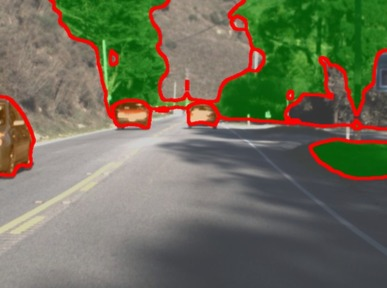
\includegraphics[width=.3\textwidth]{fps_s_1}}
        \subfigure[风格图片]{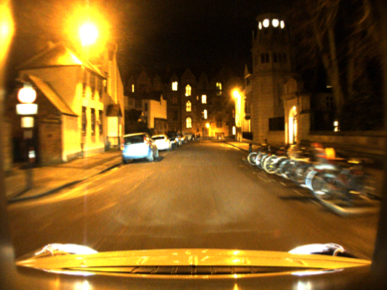
\includegraphics[width=.3\textwidth]{fps_s_3}}
        \subfigure[合成图像]{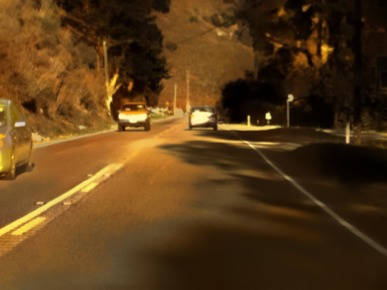
\includegraphics[width=.3\textwidth]{fps_s_2}}
        \caption{EBGAN语义分割合成图}
        \label{fig:seg}
    \end{figure}

    从另一个角度考虑,也许方向盘拐角偏差大的合成图对于DeepRoad测试框架而言,没有拐角偏差小的合成图的应用价值大,但是对于自动驾驶的另一类测试系统,比如针对自动驾驶系统作对抗攻击的测试框架应用价值却很大,比如MUNIT的合成图就很适合作为对抗攻击测试框架的测试用例。由之前章节的介绍我们知道MUNIT同样存在大量效果比较好的合成图,拐角偏差体现出MUNIT合成图对自动驾驶系统较大的干扰性使得它可以作为一个很好的对抗攻击测试用例生成技术。 
\end{enumerate}

\section{定性发现分析}

前一小节介绍了我们在对3个评价指标实验数据收集且观察后,直接基于实验数据做了定量分析并总结了3个结论。此外,我们还对实验数据中出现的一些特例和现象也做了以下的定性分析。

\begin{enumerate}[itemindent=40pt, listparindent = 0.7cm, label={发现\arabic*:}]
    \setcounter{enumi}{3}
    \item \textbf{内容图像数据集和风格图像数据集在语义上的相关性对合成图的质量有很大影响}
    
    我们对实验的8个模型所有的合成图进行观察后发现,模型最后的合成图像都对模型的训练数据十分敏感,其中MUNIT最为显著,图\ref{fig:g-munit}为MUNIT官方实验样例图,文献\cite{MUNIT}指出,在其使用的训练集中,内容图片集与样式数据集中图片的内容十分接近。从图\ref{fig:g-munit}中可以看出路况场景的合成图与真实的路况场景十分接近,与前文给出的在我们自己的路况数据集上,使用相同的算法和配置参数实验的合成图质量相比,要好很多。由于图\ref{fig:g-munit}中的合成图模型训练数据集使用的是NVIDIA提供的闭源数据,所以我们没能复现其示例中的实验结果。
    
    \begin{figure}[]
        \centering
        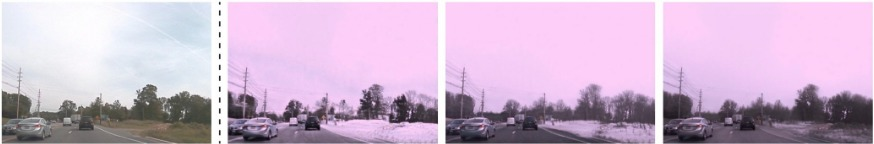
\includegraphics[width=.8\textwidth]{results/good/munit-g-1}
        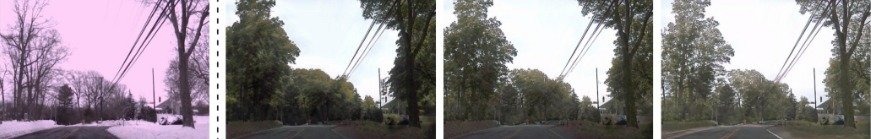
\includegraphics[width=.8\textwidth]{results/good/munit-g-2}
        \caption{MUNIT官方给出的路况场景合成样例图}
        \label{fig:g-munit}
    \end{figure}

    由于现实场景中寻找一组语义相近的内容图集和风格图集很困难,且我们在Youtube上收集的数据以及从各大开源数据集中收集的路况图像都与实验中的内容数据集,即Udacity路况数据集在语义上都有不小的差异,所以最终的实现效果较示例中的效果要差很多。这点从之前的实验结果样例图中可以很清晰的看出。 

    因此,我们认为在自动驾驶系统测试用例的自动生成,或者一般性的图像风格转换工作中,如果想要最终获得效果令人满意的合成图,那么无论采用的是对抗生成网络技术还是需要训练模型的神经风格迁移技术,训练数据集,即内容图片集和风格图片集至关重要,甚至直接影响了图像的最终合成效果。此外,通过比较我们的实验结果和模型的官方合成效果极其训练数据集,不难看出在进行图像风格转换过程中,内容图像集和风格图像集的图像结果和内容应尽可能的接近,甚至建议在选择图像集前,对内容图像集和风格图像集进行一次FID值计算,以此来量化两者的相近程度。这一点我们也考虑添加到后续研究中,以此来证实内容图像集与风格图像集的相近程度是否与模型的最终合成图成像品质成正比。但从已有的数据中我们对于这个结果还是持肯定态度的。

    \item \textbf{对抗生成网络模型在图像风格转换的应用上,很容易将风格图像的内容特征重构到最终的合成图中}
    
    \begin{figure}[h]
        \centering
        \subfigure[出现新物体的GAN合成图]{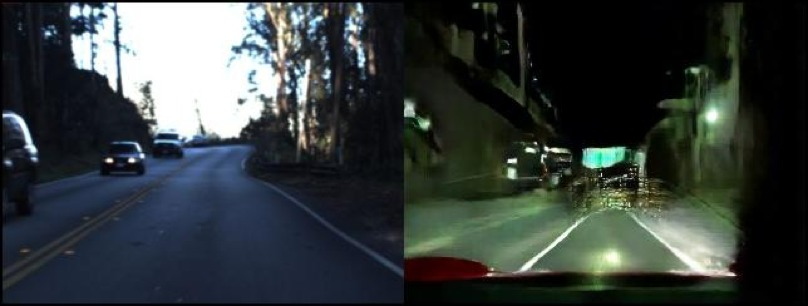
\includegraphics[width=.75\textwidth]{gan_n}}
        \subfigure[典型的神经风格迁移合成图]{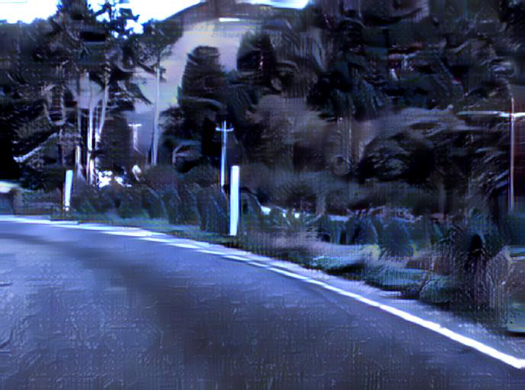
\includegraphics[width=.5\textwidth]{nst_n}}
        \caption{合成图效果对比}
        \label{fig:new}
    \end{figure}

    在仔细查看所有模型的最终合成图后我们发现,相比图像转换技术,对抗生成网络的合成图片中,会新增有很多样式图片集中特有,而原图像没有的元素。新出现的元素或物体常常属于风格图片集中的物体,比如图\ref{fig:new}所示,右边合成图中间出现了本属于风格图像集中的街景物体,从图片整体上来看,合成图的整体图像风格以及图形语义结构似乎更接近于风格图像集了。相较原图,合成图完整的保留了道路的图像内容,而原图中的车辆树木在合成图中都消失了。对比神经风格迁移技术的合成图片,典型的如图\ref{fig:new}中下图所示,合成图图像内容上几乎和原图是保持一致不变的,物体的减少和新增的情况很少出现。且图像转换技术合成的图片中,主要针对的是对远图像中像素的颜色通道和明暗值做修改,这跟对抗生成网络类的模型有很大的不同。从这一点上,神经风格迁移技术相较对抗生成网络技术更贴近风格转换的功能需求。

    \item \textbf{变分自编码技术对语义复杂的图像特征的提取和学习能力有限}

    虽然目前变分自编码器技术被广泛地应用在了图像合成应用中,但大部分实现该技术的模型都是基于一些语义较为简单的图像合成,比如MNIST数字数据集,CelebA人脸数据集。对于这一类的图像,我们希望编码器主要学习提取的特征非常明确且单一,即数字特征和人脸特征,但对于路况数据集而言,我们期望模型学习的特征则相对复杂且多样,比如最重要的是路况的道路信息,车辆信息以及路边的各种交通指示信息,比如红绿灯信号等等。对于这种包含语义极为复杂的图像,变分自编码技术不能做到很好的特征提取和特征学习\cite{vae}。
    
    \begin{figure}[h]
        \centering
        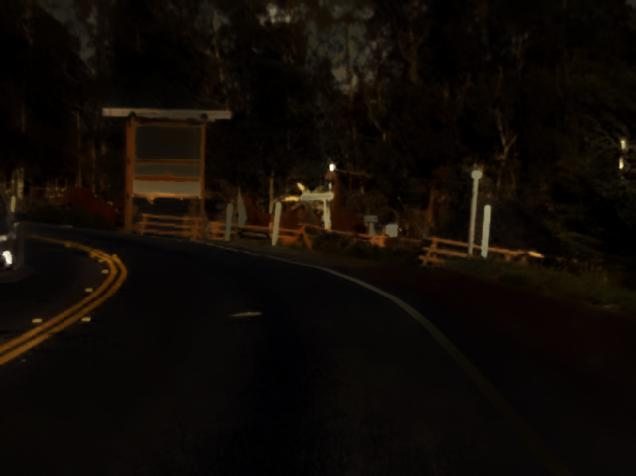
\includegraphics[width=.23\textwidth]{fps/night}
        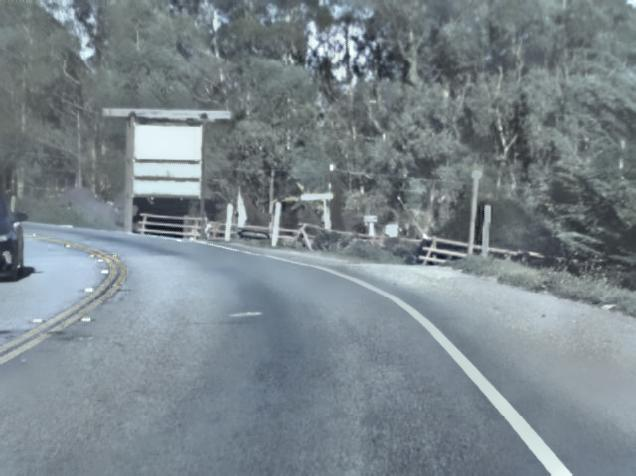
\includegraphics[width=.23\textwidth]{fps/snow}
        \includegraphics[width=.23\textwidth]{backups/1}
        \includegraphics[width=.23\textwidth]{backups/2}
        \caption{Fast Photo Style合成图对比}
        \label{fps:com}
    \end{figure}

    在前文介绍的神经风格迁移技术中,多数都利用了变分自编码技术进行最终的图像合成,典型的有Fast Photo Style。如图\ref{fps:com}所示,左边2幅图的原图重要的内容特征仅有路牌、树木和路面,而右边的还有车辆,路灯等其它特征。而前者对现实的路况场景还原度也明显比后者的高。

\end{enumerate}